\section{Fischia}\label{fischia}

Tags: Città, Luogo Creatore: Davide

\section{Fischia}\label{fischia-1}

\begin{center}\rule{0.5\linewidth}{0.5pt}\end{center}

\begin{figure}
\centering
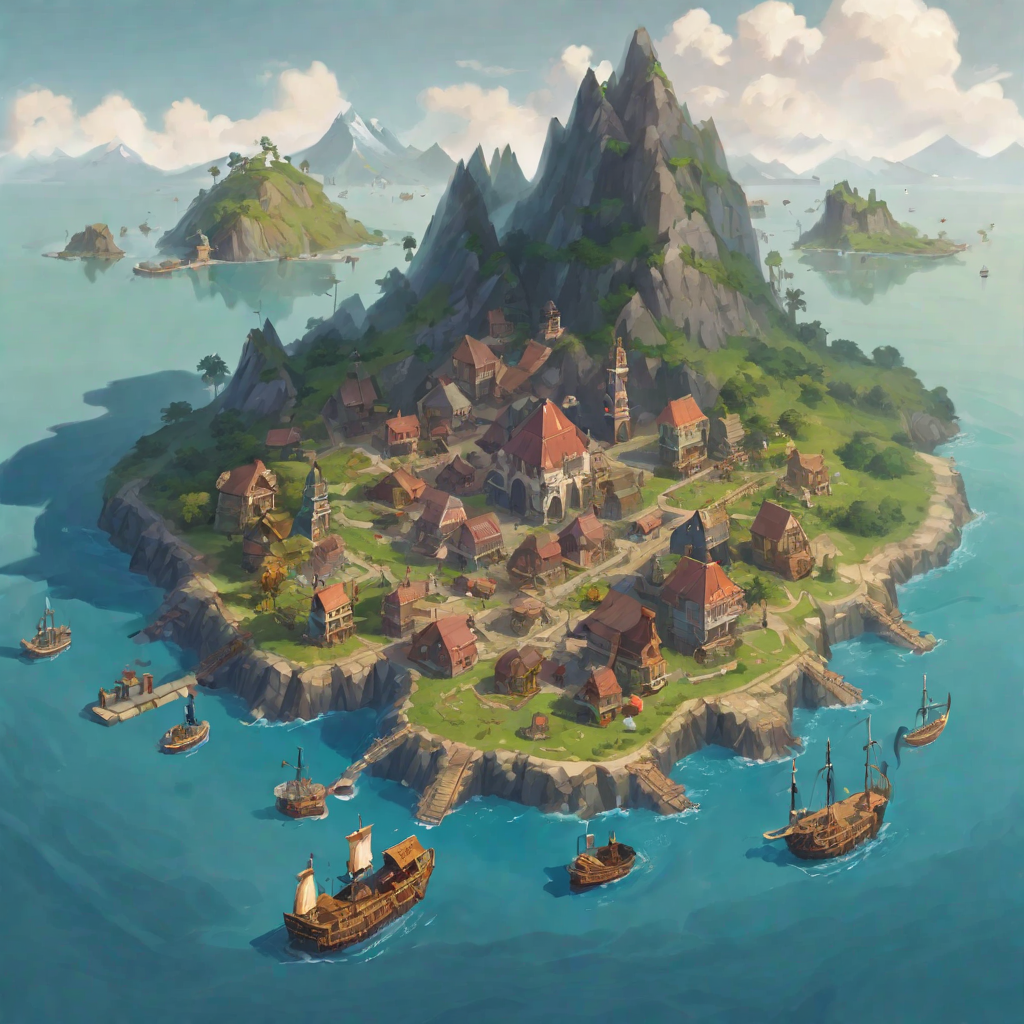
\includegraphics{a-small-island-with-a-town-in-it-it-has-a-port-with-several-mercantile-and-pirate-ships-the-island-346716834.png}
\caption{a-small-island-with-a-town-in-it-it-has-a-port-with-several-mercantile-and-pirate-ships-the-island-346716834.png}
\end{figure}

Informazioni Generali

Tipo di Luogo: Isola

Dimensioni:

Altitudine: 600 m slm

Popolazione:

Paese: Azura

Luogo:

Alleata con: Azura

Attività: Commercio, turismo

\begin{center}\rule{0.5\linewidth}{0.5pt}\end{center}

\subsection{1. Descrizione Generale}\label{descrizione-generale}

\begin{center}\rule{0.5\linewidth}{0.5pt}\end{center}

\begin{figure}
\centering
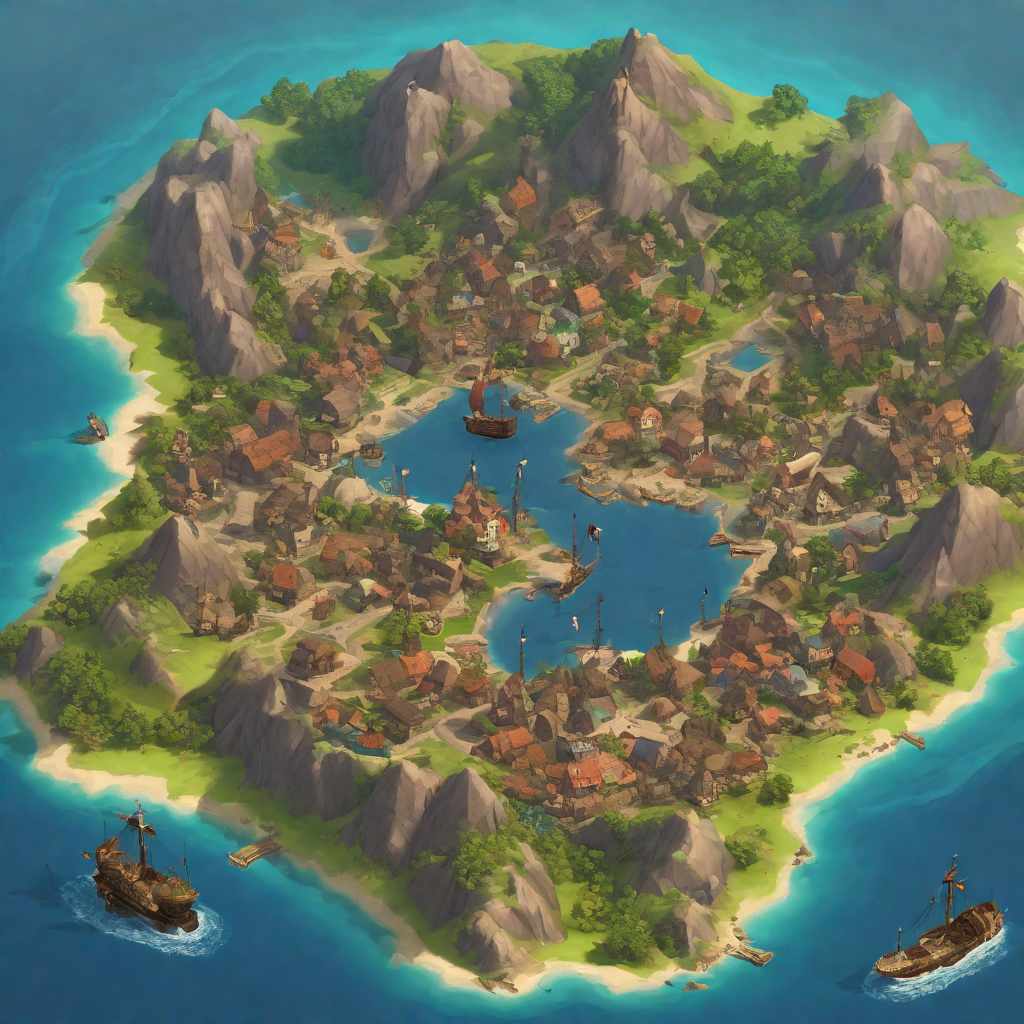
\includegraphics{a-small-island-with-a-town-in-it-it-has-a-port-with-several-mercantile-and-pirate-ships-the-island-744785231.png}
\caption{a-small-island-with-a-town-in-it-it-has-a-port-with-several-mercantile-and-pirate-ships-the-island-744785231.png}
\end{figure}

L'Isola di Fischia è una pittoresca isola situata nel cuore del Mare di
Smeraldo, famoso per le sue acque cristalline e la bellezza naturale
mozzafiato. Caratterizzata da una posizione strategica nello stretto
marittimo della regione, l'isola è amministrata dalla maestosa città di
Azura, situata a breve distanza di navigazione. Il nome dell'isola
deriva dalla sua orografia unica, che durante giornate ventose genera
melodie simili a fischi, creando un'atmosfera magica.

\subsection{2. Storia}\label{storia}

\begin{center}\rule{0.5\linewidth}{0.5pt}\end{center}

L'Isola di Fischia, con la sua storia avvincente e stratificata, ha
sempre affascinato gli storici e gli appassionati di archeologia. Le
prime tracce umane risalgono a tempi antichissimi, con reperti
archeologici che testimoniano la presenza di una civiltà preistorica che
si insediò sull'isola migliaia di anni fa. Questi antichi abitanti, noti
come gli ``Scopritori del Vento'' per la loro venerazione dei suoni
prodotti dal vento tra le montagne, hanno lasciato dietro di sé
incisioni rupestri enigmatiche e misteriosi siti cerimoniali che sono
tuttora oggetto di studio e di ammirazione.

Nel corso dei secoli successivi, l'Isola di Fischia fu teatro di
molteplici culture e dominazioni. Durante l'epoca medievale, fu contesa
tra regni rivali alla ricerca di posizioni strategiche nel Mare di
Smeraldo. I forti e le torri di avvistamento costruiti su promontori
rocciosi testimoniano la lotta per il controllo dell'isola.

Tuttavia, uno dei capitoli più importanti della storia di Fischia ebbe
inizio quando l'imponente città di Azura la reclamò come proprio
possedimento nel XVIII secolo. L'isola divenne rapidamente una
postazione marittima cruciale per Azura, con il porto di Fischia che si
sviluppò rapidamente per accogliere le navi mercantili provenienti da
ogni angolo del mondo. La prosperità economica e culturale che ne derivò
trasformò l'isola in un gioiello di bellezza e diversità.

Nel corso dei secoli, l'amicizia tra l'Isola di Fischia e Azura si è
consolidata, portando a una lunga era di stabilità e cooperazione. Azura
ha contribuito alla conservazione del patrimonio storico dell'isola,
restaurando antichi siti e proteggendo le tradizioni locali, mentre
l'isola ha fornito risorse naturali e beni di lusso che hanno arricchito
la città madre.

Oggi, l'Isola di Fischia è un esempio vivente di come la storia e la
modernità possano coesistere armoniosamente. Gli abitanti dell'isola
onorano il loro passato celebrando le tradizioni antiche, mentre si
abbracciano le opportunità del futuro. Il legame indissolubile tra
Fischia e Azura continua a prosperare, garantendo un futuro luminoso per
questa affascinante isola nel cuore del Mare di Smeraldo.

\subsection{3. Geografia}\label{geografia}

\begin{center}\rule{0.5\linewidth}{0.5pt}\end{center}

L'Isola di Fischia è un gioiello geografico circondato dalle acque
turchesi del Mare di Smeraldo. La sua topografia è caratterizzata da
maestosi monti che attraversano l'isola, creando una serie di valli e
piccole pianure. Questi monti, noti per il loro contributo ai fischi
melodiosi durante le giornate ventose, sono coperti da foreste
lussureggianti e arricchiti da flora e fauna uniche.

\subsection{4. Economia}\label{economia}

\begin{center}\rule{0.5\linewidth}{0.5pt}\end{center}

L'economia dell'Isola di Fischia è strettamente legata al commercio
marittimo, grazie alla sua posizione strategica nello stretto marittimo.
Le principali fonti di reddito includono il commercio di merci
provenienti da tutto il mondo, la pesca abbondante grazie alle acque
ricche di vita marina e il turismo, attratto dalle bellezze naturali
dell'isola e dalla sua cultura unica. I mercati locali abbondano di
prelibatezze ittiche, prodotti agricoli freschi e artigianato locale,
contribuendo alla prosperità dell'isola.

\subsection{5. Cultura}\label{cultura}

\begin{center}\rule{0.5\linewidth}{0.5pt}\end{center}

L'Isola di Fischia è un crocevia di culture grazie al suo passato di
dominazioni diverse. La cultura locale riflette questa diversità, con
influenze culinarie, artistiche e musicali provenienti da tutto il
mondo. Gli abitanti dell'isola sono noti per la loro ospitalità e il
loro orgoglio per le tradizioni locali. Artisti locali dipingono
paesaggi ispirati alla bellezza naturale circostante, mentre i musicisti
si esibiscono nei caratteristici suoni dei fischi melodia durante le
giornate ventose.

\subsection{6. Governo}\label{governo}

\begin{center}\rule{0.5\linewidth}{0.5pt}\end{center}

L'Isola di Fischia è amministrata da Azura, una città marittima di
risonanza che ha garantito stabilità e sicurezza all'isola negli ultimi
due secoli. Il governo locale opera sotto la guida di un sindaco eletto
democraticamente, che collabora strettamente con le autorità di Azura
per gestire le questioni amministrative e promuovere lo sviluppo
sostenibile dell'isola. La collaborazione tra l'isola e la città madre
ha portato a una cooperazione efficace nei settori dell'educazione,
della sanità e dell'infrastruttura, garantendo un elevato standard di
vita per gli abitanti di Fischia.

\begin{center}\rule{0.5\linewidth}{0.5pt}\end{center}
